\section{Dashboard}\label{sec:12}

The operator view has two halves, deliberately.

\textbf{On BuildSim's own viewer}, \texttt{dashboard} repaints all four layers every 5 s, and a
query parameter switches which one the rooms are coloured by. The viewer offers a 3D mode and a
floor plan; \textbf{every capture in this report is the plan}, deliberately. It shows all six
rooms and which one has gone red in a single frame, where a perspective render hides whichever
rooms are behind the near wall. The layer being painted is the same either way: the colouring is
\texttt{dashboard}'s, pushed through BuildSim's room-layer API, and the view toggle is the
operator's.

\begin{longtable}[]{@{}
  >{\raggedright\arraybackslash}p{(\columnwidth - 6\tabcolsep) * \real{0.15}}
  >{\raggedright\arraybackslash}p{(\columnwidth - 6\tabcolsep) * \real{0.14}}
  >{\raggedright\arraybackslash}p{(\columnwidth - 6\tabcolsep) * \real{0.26}}
  >{\raggedright\arraybackslash}p{(\columnwidth - 6\tabcolsep) * \real{0.45}}@{}}
\toprule
\textbf{Layer} & \textbf{Range} & \textbf{Why that range} & \textbf{What it shows the operator} \\
\midrule
\endhead
\texttt{co2} & 420–1500 ppm & Outdoor level to half again the comfort limit & The air, which is what
occupants feel\\*
\texttt{residual} & $-100$ to $+500$ ppm & The spike measured healthy residuals spanning $-76.5$ to
$+80.3$ ppm and a stuck damper's post-command mean at 507.8 ppm, so the scale is set by measurement
rather than by taste & How far the room is from what its command owed\\*
\texttt{cusum} & 0–300 ppm & Twice $h$, so the limit sits at mid-scale & How close the room is to
confirmation\\*
\texttt{state} & 0–3 & latched 3, stale or \texttt{BLIND} 2, \texttt{SUSPECT} 1, else 0 & The
equipment, which is not the same thing as the air \\
\bottomrule
\end{longtable}

The \texttt{state} layer is the interesting one and it exists for one reason: \textbf{it keeps a
latched room hot after compensation has pulled its residual back to zero.} On the \texttt{co2} and
\texttt{residual} layers a compensated room looks healthy (which is true of the air and false of
the equipment), and the severity ordering is chosen precisely so that the latched room stays the
hottest thing on the floor. The same concern shapes the projection behind the view: only an explicit
fault-state event moves a room's monitor state, so the arrival of small residuals, which is exactly
what successful compensation produces, cannot talk the display out of a diagnosis the monitor
latched.

A stale measurement is painted at the layer minimum rather than frozen at its last value, because
BuildSim's layer API carries numbers and a range with no no-data sentinel; \texttt{state} is exempt
because it is not a measurement. And \texttt{dashboard} \textbf{never writes a BuildSim alert}:
alerts are a whole-collection PUT, so a second writer would erase the supervisor's work orders
rather than add to them. One writer per resource, for the same reason one component commands.

\textbf{Beside it}, a server-rendered HTML table at port 8080 (no JavaScript, no framework, no
CDN, just a meta refresh every 5 s) with \texttt{GET /api/state} serving the same view as JSON and
\texttt{GET /api/cases/\{caseId\}} replaying one diagnosis out of the journal, which is R-5's
interface and not a convenience. The replay is encoded with the same codec that published the
events, so a replay cannot disagree with what went over the wire, and its failure modes are
distinguished rather than collapsed: 400 for a blank id, 404 for an unknown case, and 503 with
\emph{different detail text} depending on whether the journal is unconfigured or configured but
unreachable.

Every dependency of this page is optional, and that is a deliberate inversion of the usual
dependency direction for a dashboard: it keeps serving when the broker, BuildSim or the database is
down, retrying each on its 5 s tick, which makes it the instrument for telling whether the rest of
the system is alive. Its health probe is never reported DOWN for the same reason: a dashboard that
failed readiness because no readings were arriving would be restarted by the orchestrator at
precisely the moment an operator needed to look at it. The price is a little duplicated
state-handling and a page that can show a confidently empty table.

\begin{center}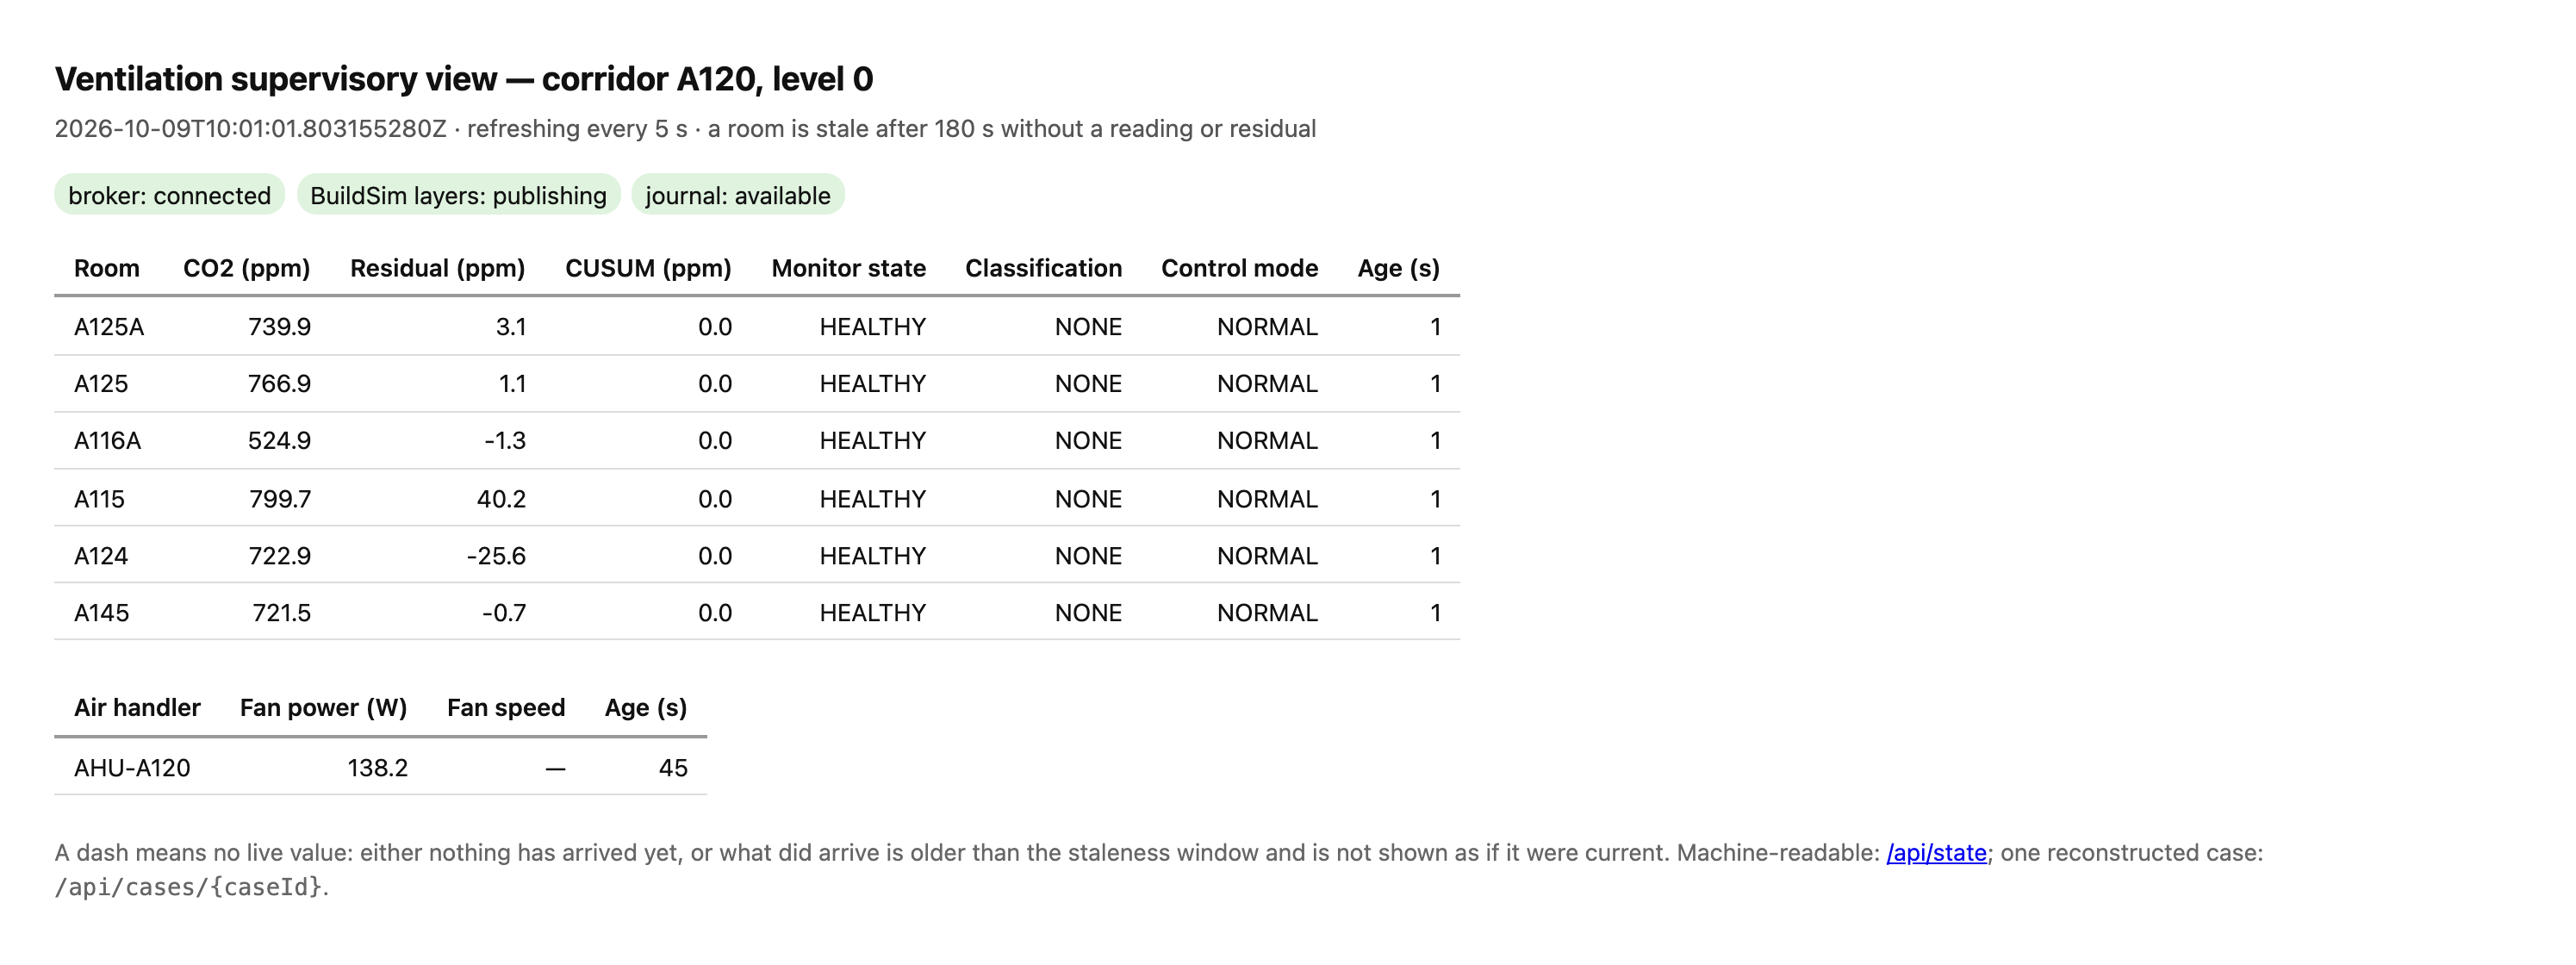
\includegraphics[width=\linewidth]{screenshots/dashboard-not-firing.png}\end{center}
\figcap{Simulated 10:01:01, 46 simulated minutes after the damper jammed. A115 has climbed to
799.7~ppm and its residual is \textbf{+40.2~ppm}, while its CUSUM is still \textbf{exactly 0.0}
and every room reads \texttt{HEALTHY}. This is the frame worth defending against ``your detector
is only a threshold'': a threshold placed anywhere below 40~ppm would have fired here. The CUSUM
has not accumulated because it is not driven by this column: \texttt{ZoneMonitor} advances it
on the \emph{occupancy-plausible} residual, measured minus the prediction's \emph{ceiling}, so the
table's residual and the detector's input are two different series (§\ref{sec:11}, ADR-0010). The fan speed
shows an em-dash because no live value had arrived yet, which is the no-stale-number rule in
Section \ref{sec:12} acting rather than a gap.}

Three further frames are in \textbf{Appendix \ref{sec:H.1}}: the same table with A115 \texttt{CONFIRMED} at
simulated 10:23:27, with the other five rooms \texttt{HEALTHY} at CUSUM 0.0, R-7's isolation
visible in one frame; BuildSim's own floor plan
beside the work order the \emph{supervisor} PUT, naming the diagnosis, the action taken and the bound
the plan ran into; and corridor A120 painted by all four layers at one instant with A115 latched and
\texttt{COMPENSATING}. That last figure is this section's argument measured rather than asserted:
compensation has done its job, so on \texttt{co2} the broken room is the second coolest on the floor
and on \texttt{cusum} it is indistinguishable from five healthy rooms, and only \texttt{state} still
says the equipment is broken.

What the figures do \emph{not} settle is what the view \emph{must} show: no requirement states it,
so these are evidence that the operator path works end to end, not evidence against a criterion.

\subsection{Two defects the capture found, and one limit it exposed}\label{sec:12.1}

Capturing those frames found two defects and exposed one limit, and \textbf{Appendix \ref{sec:H.2}} reports all
three in full. \textbf{The layers were overwriting each other}: \texttt{/api/room-layers} is a
collection endpoint whose PUT replaces the whole collection, and the dashboard was publishing its
four layers one at a time, so each call erased the one before it and only the last layer of the enum
ever reached BuildSim, with every individual PUT returning 200, so nothing anywhere said so. The
fix sends every layer on every call, and the run above confirms it against the real stack:
\texttt{GET /api/room-layers} returns \textbf{four layers of six zones each}. \textbf{A compensated
room is painted exactly like a dead sensor}, because $-100$ is both the bottom of the
\texttt{residual} scale and the only no-data encoding BuildSim's layer API offers; that is recorded
as a limit rather than patched, for a reason the appendix gives. And \textbf{\texttt{SUSPECT} cannot
be photographed}: a 1~Hz poll of \texttt{/api/state} caught A115 in it in \textbf{2 of 295 usable
samples} against a page that refreshes every 5~s, so that state is evidenced from the
\texttt{decisions} journal and from the poller instead, and the screenshots are taken only at states
that latch.
